\chapter{Effets de taille finie}
    \label{chap-sos}

disjoining pressure
\cite{bergeron_forces_1999}
\cite{stubenrauch_disjoining_2003}



Certains dépôts de films nanoscopiques sur des surfaces présentent des fluctuations dont la longueur de corrélation est similaire à celle de la hauteur du film. L'interface entre le dépôt et le substrat présente une énergie libre qui dépend fortement de la taille dudit film\cite{ouyang_size-dependent_2006,jiang_size_2008}. De telles modifications des propriétés thermodynamiques à cause d'un effet de taille finie peut provoquer de fortes instabilités hydrodynamiques pouvant rendre le système thermodynamiquement instable\cite{ding_theoretical_2001}. Ces conditions aux limites entraînent une frustration du système qui finit par causer une force entre les surfaces du système, appelé force Casimir. Cette force entropique peut se retrouver dans les systèmes critiques et possède alors des propriétés universelles selon la classe d'universalité du système. Plus proche des dépôts de film on retrouve les systèmes de membranes\cite{nelson_statistical_2004} possédant une force non-universelle\cite{hasnaoui_casimir_2010}. Certaines membranes biologiques possèdent même une transition de phase appartenant à la classe d'universalité du modèle d'Ising \cite{machta_critical_2012}.

Dès lors, quelles propriétés de la force de Casimir peut-on retrouver dans un modèle Solid-On-Solid d'Hamiltonien
\begin{align}
    \mH = J \sum_i |h_i-h_{i+1}| + \mu \frac{h_i+h_{i+1}}{2}
\end{align}
et avec quels outils peut-on l'étudier ?

%%%%%%%%%%%%%%%%%%%%%%%%%%%%%%%
\section{Limite thermodynamique}
%%%%%%%%%%%%%%%%%%%%%%%%%%%%%%

De la densité de probabilité de l'interface découle toutes les propriétés thermodynamiques du système comme la magnétisation moyenne ou l'énergie libre. Lorsque la taille $L$ du système change, les hauteurs supérieures à $L$ ne sont plus disponibles, et on voit un tassement de la distribution. Dans le régime thermodynamique, c'est-à-dire où l'on suppose que la taille $L$ est nettement supérieure à la largeur de la distribution, le mode des fluctuations de plus basse énergie suffit à expliquer les propriétés thermodynamiques \footnote{Pour rappel, la fonction de partition est calculée par $\mZ = \sum_i \lambda_i^L$, avec $\lambda_0 \greater \lambda_i$ le mode de plus basse énergie (équation \ref{partition-trace-lambda}).}. Lorsque la taille du système diminue, l'énergie de tous les modes de fluctuations changent, et la puissance dans la fonction de partition pénalise moins fortement les modes suivants. 

On considère l'approximation thermodynamique vraie lorsque les propriétés du système sont indépendantes de la taille du système. Le système cesse d'être contraint par les conditions aux bords lorsque $\xi \ll L$. En dehors de cette limite, on peut alors s'attendre à des effets de taille finie, notament l'effet Casimir.

\begin{figure}
	\begin{minipage}[t]{0.4\linewidth}
		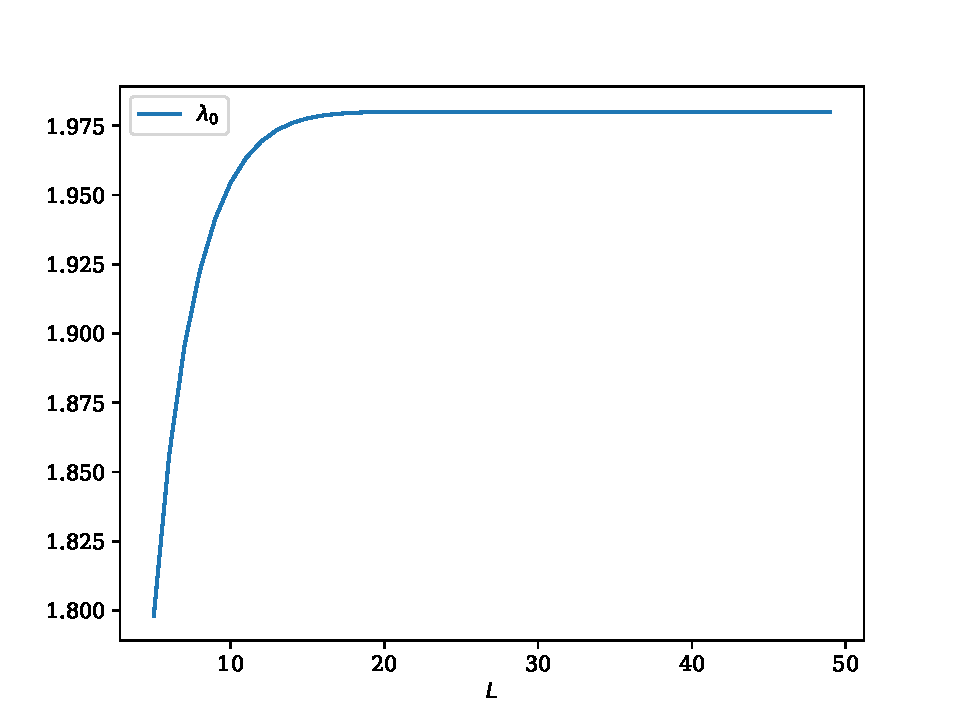
\includegraphics[width=\linewidth]{chap4/freeene-lambda0-mu.pdf}
	\end{minipage}%Cyclin
	\begin{minipage}[t]{0.4\linewidth}
		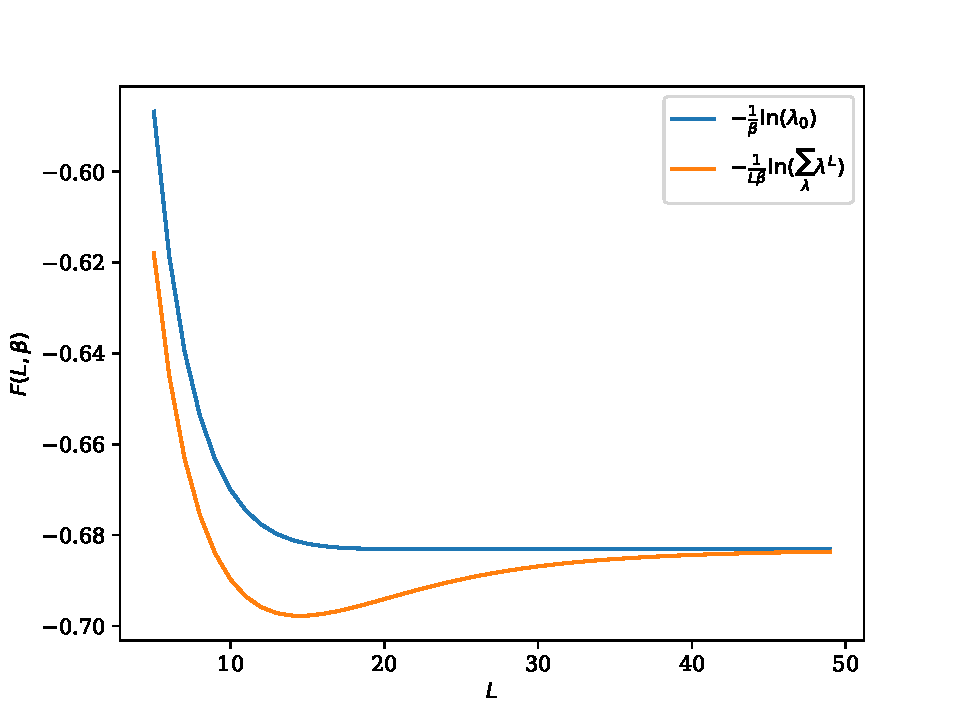
\includegraphics[width=\linewidth]{chap4/freeene-thermo-mu.pdf}
	\end{minipage}
	\begin{minipage}{0.4\linewidth}
    	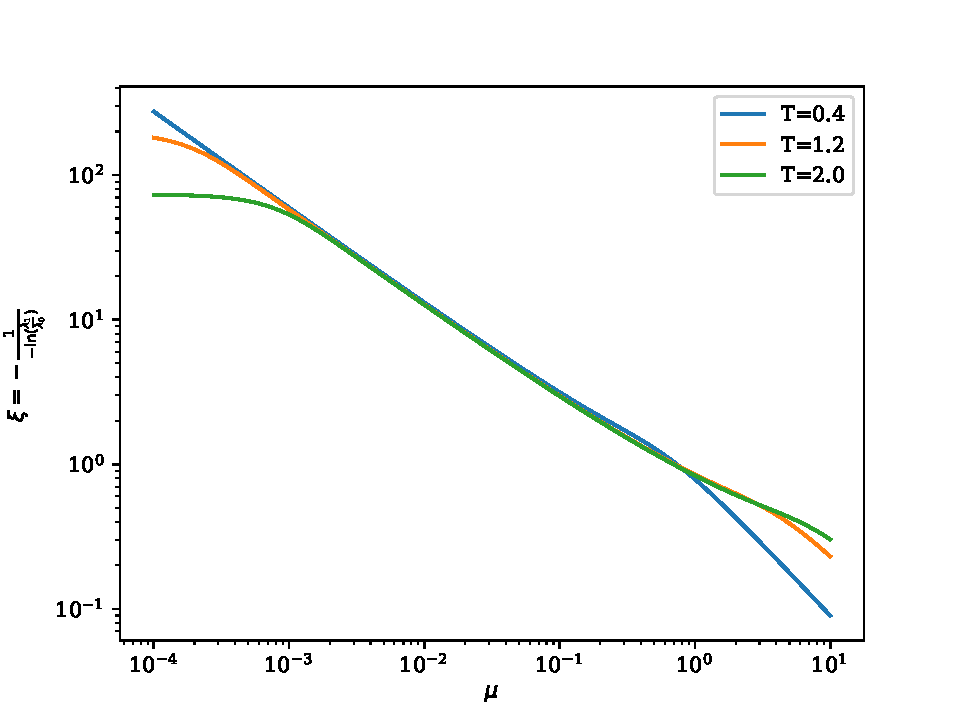
\includegraphics[width=\linewidth]{chap4/longueur-correl.pdf}
	\end{minipage}
	\begin{minipage}{0.4\linewidth}
    	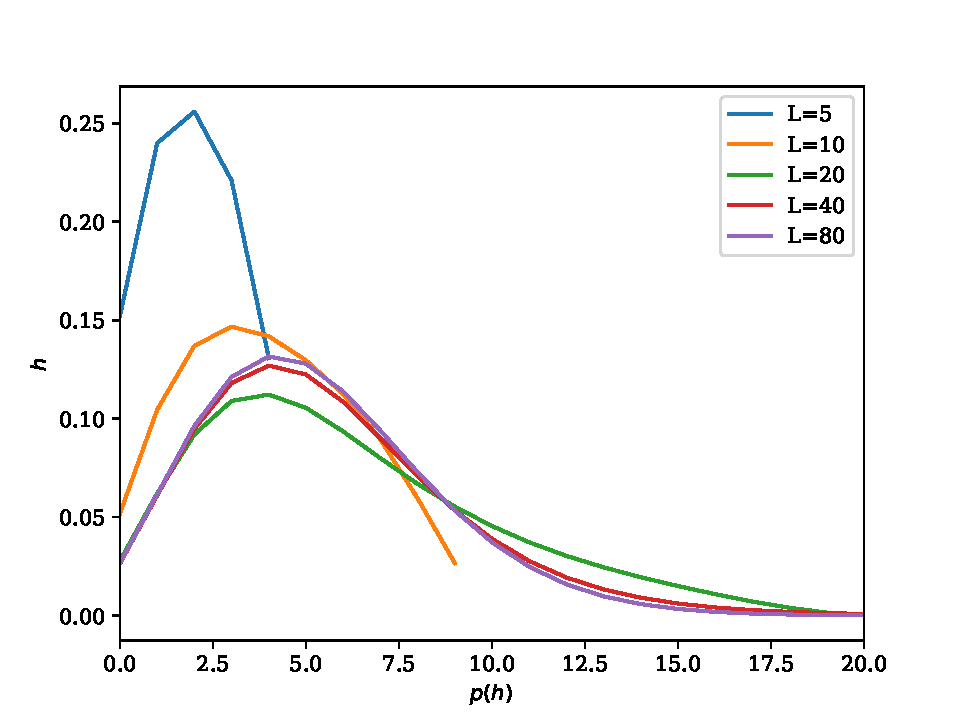
\includegraphics[width=\linewidth]{chap4/distribution-taille-finie.pdf}
	\end{minipage}	
	\caption{Plus grande valeur propre d'une interface libre en fonction de la taille $L$ du système pour $\mu = 0.01$ et $\beta = 1$ (haut gauche)  ; énergie libre par site calculée via l'approximation de la limite thermodynamique \ref{energie-libre-site} comparé à la vraie fonction de partition \ref{partition-trace-lambda} en fonction de la taille $L$ du système pour $\mu=0.01$ et $\beta = 1$ (haut droite) ; longueur de corrélation à grande distance \ref{longueur-correl-thermo} pour une matrice $200\times200$ en fonction du potentiel chimique $\mu$ pour différentes températures (bas gauche) ; distribution de l'interface pour différentes tailles de la matrice de transfert à $\mu=0.01$ et $\beta = 1$. Par un fit, la distribution ne suit pas une distribution de Poisson (bas droite) .}
	\vspace{-0.5cm}
\end{figure}  


%%%%%%%%%%%%%%%%%%%%%%%%%%%%%%%%%%
\section{Effet Casimir}
%%%%%%%%%%%%%%%%%%%%%%%%%%%%%%%%%%

Dans la section \ref{sec-casimir} nous avons introduit l'effet Casimir comme étant le surplus d'énergie libre causé par le confinement du système, soit 
\begin{align}
    f_c(\beta,L,h) = - k_B T \frac{\partial(L \omega_{ex}(\beta,L,h))}{\partial L}\bigg|_{\beta,L'}
\end{align}
où $\omega_{ex}$ est l'énergie libre en excès dans le système, et prend une forme universelle proche du point critique. Cet excès d'énergie libre est dûe à la frustration du système lorsque la longueur de corrélation est du même ordre de grandeur que la taille du système. Afin d'obtenir cette quantité dans les modèles sur réseau à partir de l'énergie libre totale, il est nécessaire de soustraire l'énergie du bulk au total. Néanmoins, dans les modèles d'interfaces qui nous intéressent, le seul terme extensif contribuant à l'énergie libre est l'énergie de surface, qui disparaît lorsque l'on prend la dérivée par rapport à la taille du système. Il n'est donc pas nécessaire de comparer l'énergie libre à la limite thermodynamique, et on obtient directement la force de Casimir
 \begin{align}
    f_c(\beta,L,h) = - \frac{\partial \Omega}{\partial L}\bigg|_{\beta} = k_B T \frac{\partial \ln Z(\beta,\mu,L)}{\partial L}
    \label{casimir-interface}
\end{align}
Il est difficile de se faire une vision claire de l'effet Casimir, parce que le modèle Solid-On-Solid n'étant pas critique, il ne possède pas nécéssairement de fonction universelle qui permette de réduire la dimensionalité de l'espace des phases $(\beta,\mu,L)$.

{\color{red} Comment interpréter les résultats de la figure \ref{casimir-temperature}, que dire de pertinent à leur sujet ? }
{\color{red} là on calcule une pression. Manifestation spatiale des effest de taille finie dans un système critique est casimir. 
Casimir : système de spin critique.
Là interface avec un comportement un peu de casimir, en loi de puissance des fois.
Casimir : vraie pression thermo intensive en plus pression qui dépend de la taille du système.
Colloïdes pression de disjonction. p(l)-pbulk, interaction entre les deux surfaces. \textbf{disjoining pressure}.}
\begin{figure}[t]
	\begin{minipage}[t]{0.4\linewidth}
		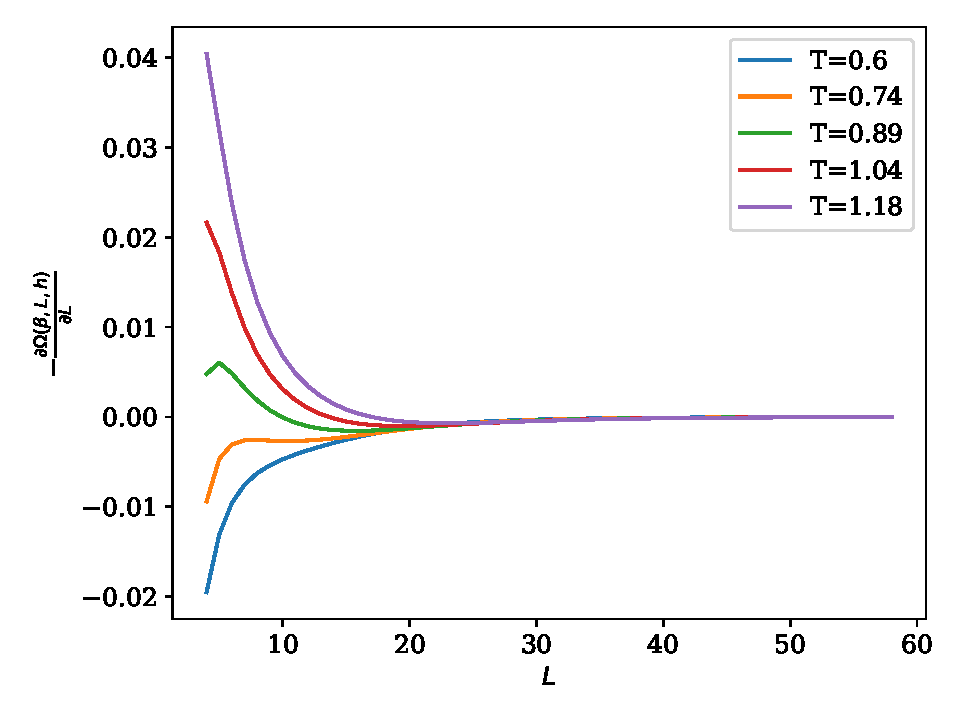
\includegraphics[width=\linewidth]{chap4/casimir-distance-mu001.pdf}
	\end{minipage}%Cyclin
	\begin{minipage}[t]{0.4\linewidth}
		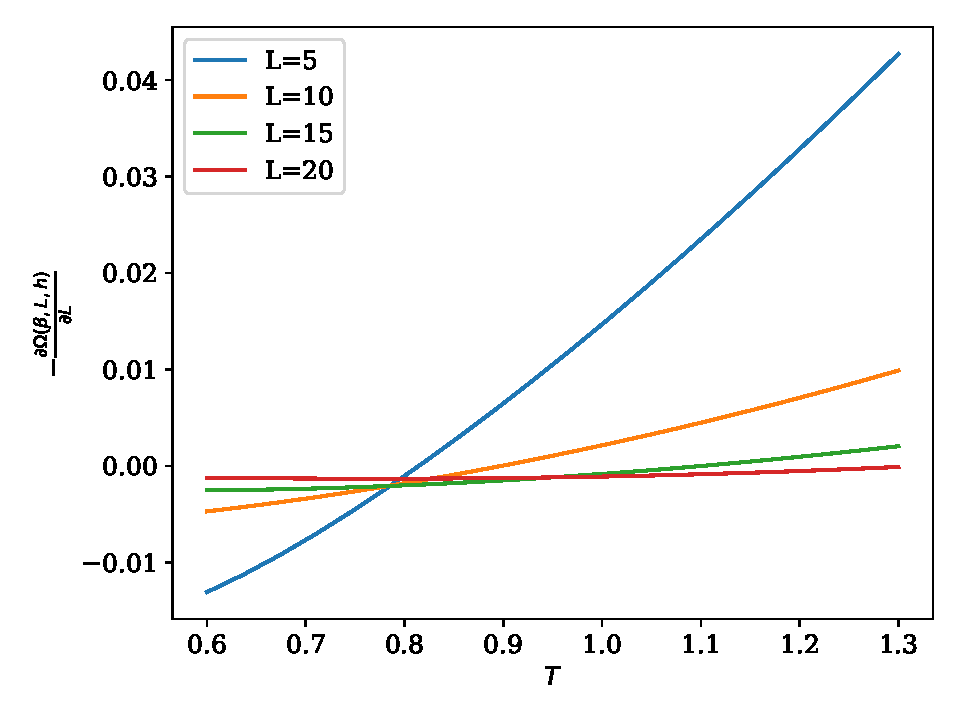
\includegraphics[width=\linewidth]{chap4/casimir-temperature-mu001.pdf}
	\end{minipage}
	\centering
	\begin{minipage}[b]{0.4\linewidth}
    	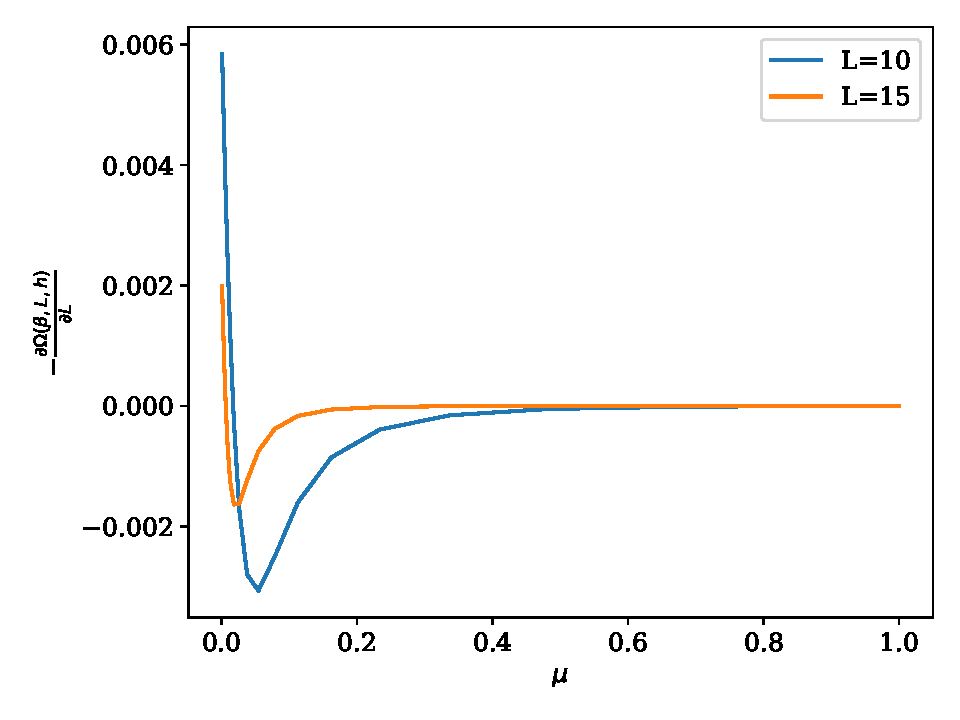
\includegraphics[width=\linewidth]{chap4/casimir-mu-t1.pdf}
	\end{minipage}	
	\label{casimir-temperature}
	\caption{Force de Casimir \ref{casimir-interface} en fonction de la distance pour $\mu = 0.01$ à température fixée (gauche) ; force de Casimir en fonction de la température pour $\mu=0.01$ à taille fixée (droite) ; force de Casimir en fonction du potentiel chimique pour différentes tailles du système à $T=1$ (bas). }
\end{figure}
    
%%%%%%%%%%%%%%%%%%%%%%%%%%%%%%%%%%
\section{Hamiltonien de transition}
\label{sec-transition}
%%%%%%%%%%%%%%%%%%%%%%%%%%%%%%%%%%
{\color{red} mettre en intro, parce que l'on ne l'utilise pas. Parler de pression thermodynaique et forces de confinement, plusieurs types de forces de confinement. }
La force de Casimir dépend  de l'énergie libre, bien qu'elle ne puisse être exprimée par des moyennes d'observables facilement calculables par Monte Carlo. Néanmoins, sa dérivée peut être calculée via la méthode du paramètre de couplage. En suivant \cite{vasilyev_monte_2007,cardozo_finite_2015} pour un système d'Ising carré de taille $L \times L'$, l'idée est de calculer la dérivée continue par rapport à une taille discrète du système $L$ en interpolant le système via l'Hamiltonien de transition
\begin{align}
    \mH_{tr}(\lambda) = (1-\lambda) \mH_0 + \lambda \mH_1
    \label{hamil-trans}
\end{align}
où $\mH_0$ est l'Hamiltonien d'un système de hauteur maximale $L$, et $\mH_1$ l'Hamiltonien d'un système de hauteur maximale $L-1$ où on a découplé une couche (voir Figure \ref{decouplage}). L'énergie libre associée à cet Hamiltonien est
\begin{align}
    \Omega_{tr}(\lambda) = -k_B T \ln \left( \sum_{h_1 ... h_L} e^{-\beta \mH_{tr}(\lambda)} \right)
\end{align}
De la dérivée de l'énerie libre découle
\begin{align}
    \frac{\Omega_{tr}(\lambda)}{d\lambda} = < \mH_1 - \mH_0>_{\mH_{tr}(\lambda)}
\end{align}
où $< · >_{\mH_{tr}(\lambda)}$ représente la moyenne statistique sur le système en transition, facilement calculable dans les simulations numériques. En intégrant sur le couplage, on trouve au final que
\begin{align}
    \Omega_1 - \Omega_0 = \int_0^1 d\lambda  < \mH_1 - \mH_0>_{\mH_{tr}(\lambda)}
\end{align}
Finalement, dans la limite où l'épaisseur du système est suffisement grande pour que la variation d'une couche soit suffisement petite ($L' \gg 1$), on trouve que
\begin{align}
   - \frac{\partial \Omega(\beta,L,h)}{\partial L} \bigg|_{\beta,L'} \simeq  \int_0^1 d\lambda  < \mH_1 - \mH_0>_{\mH_{tr}(\lambda)}
\end{align}

\begin{figure}
	\begin{minipage}[t]{0.3\linewidth}
		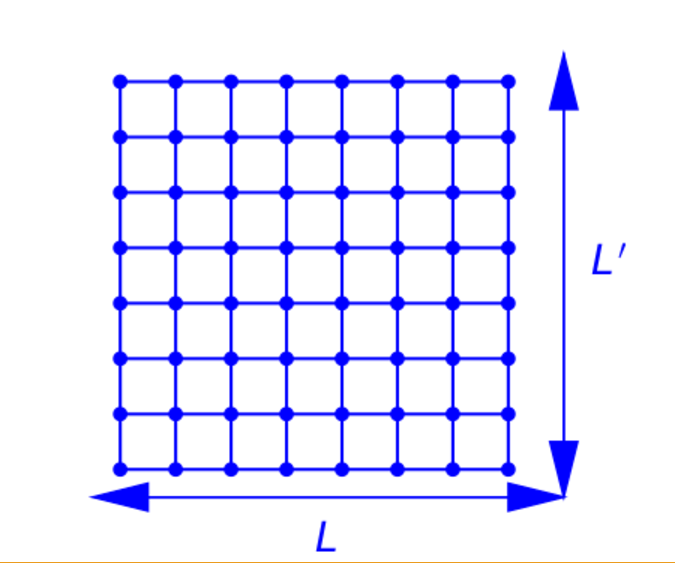
\includegraphics[width=\linewidth]{numerical/cross-h0.pdf}
		\caption*{$\mH_0$}
	\end{minipage}
	\begin{minipage}[t]{0.3\linewidth}
		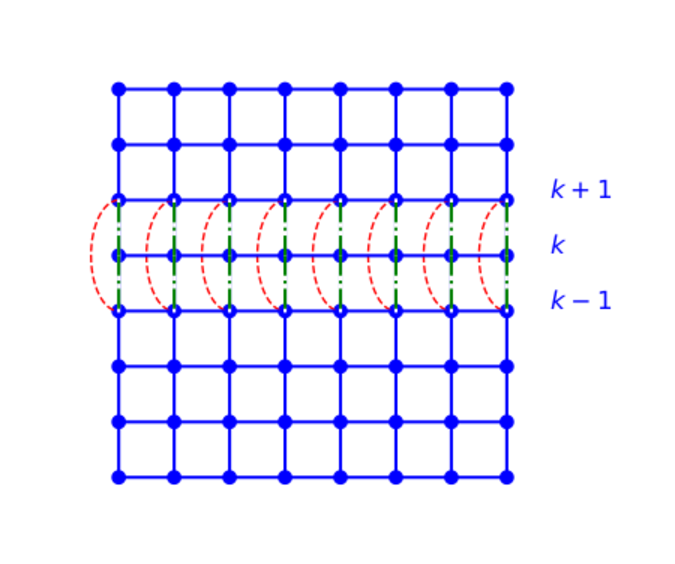
\includegraphics[width=\linewidth]{numerical/cross-hlambda.pdf}
		\caption*{$\mH(\lambda)$}		
	\end{minipage}
	\centering
	\begin{minipage}[t]{0.3\linewidth}
		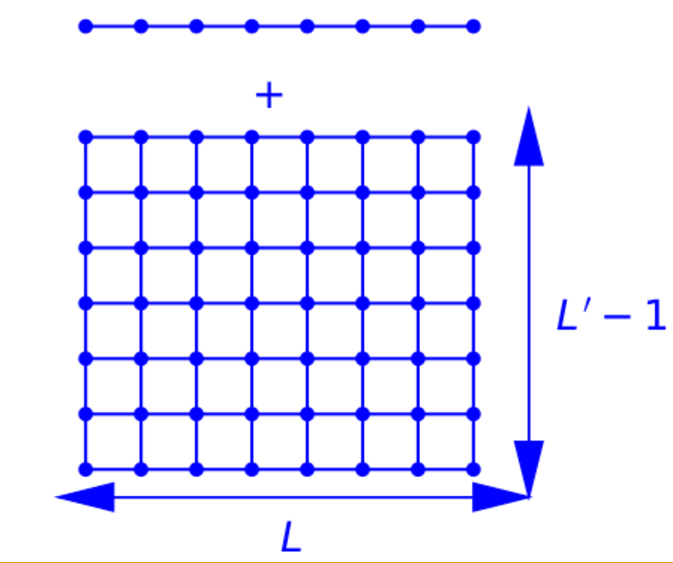
\includegraphics[width=\linewidth]{numerical/cross-h1.pdf}
		\caption*{$\mH_1$}
	\end{minipage}
	\caption{Découplage progressif de la $k$-ième couche du système afin de calculer la variation de l'énergie libre grâce à l'hamiltonien de transition. Les liens en bleu ont une énergie de $\beta J$, les liens en rouge une énergie de $\lambda \beta J $ et les liens en vert une énergie de $ (1-\lambda) \beta J$. Reproduction 2D de \cite{vasilyev_monte_2007}.}
	\label{decouplage}
\end{figure}

Pour le modèle Solid-On-Solid, il est possible de calculer la variation d'énergie créée par le découplage directement. Si le découplage s'est créé à la rangée $k$, on ajoute un lien d'énergie $\lambda J$ entre les rangées $k-1$ et $k+1$ et on retire $\lambda J$ énergie des rangées $k-1$ à $k$  et de $k$ à $k+1$. On obtient
\begin{align}
    &\mH_{tr,SOS}(\lambda) = \mH_{0,SOS} - \nn
     &\frac{\lambda J}{2} \sum_x \left[ \sgn(k-1-h(x)) \sgn(k+1-h(x)) - \sgn(k-h(x)) \left( \sgn(k-1-h(x))+\sgn(k+1-h(x)) \right) \right]
\end{align}
où le facteur $\frac{1}{2}$ est obtenu afin de prendre en compte le coefficient $2$ dans \ref{energie-sos-ising}. En faisant un tableau de valeurs, on remarque rapidement que la somme est une constante égale à $-1$ quel que soit $k$, puisque contraiement au modèle d'Ising, les modèles d'interface ne possèdent pas d'énergie de bulk. Il faut donc utiliser une autre méthode afin de mesurer l'effet Casimir dans les simulations de Monte Carlo.	
	
%%%%%%%%%%%%%%%%%%%%%%%%%%%%%%%%%%	
\section{Intégration sur le potentiel chimique}
%%%%%%%%%%%%%%%%%%%%%%%%%%%%%%%%%%
{\color{red} on saute de potentiel à champ à chaque fois
généralisation de la méthode de David pour n'importe quel observable
Contexte de David, appliqué au modèle d'Ising, dans son contexte.
PUIS traduire dans le contexte -> particule -> molécuilaire. 
 Si l'aimantation doit être conservée ça doit être adapté. Utilisation de plusieurs types de champ magnétique, nouveauté.}
Pour un système d'Hamiltonien 
\begin{align}
    \mH = J \sum_i |h_i-h_{i+1}| + \mu \frac{V(h_i)+V(h_{i+1})}{2}
    \label{potentiel-integration-param}
\end{align}
on a la différence d'énergie le long d'une isotherme entre un état de référence $(T,\mu_0)$ et $(T,\mu)$ \cite{lopes_cardozo_critical_2014}
\begin{align}
   \Omega(\beta,L,\mu) - \Omega(\beta,L,\mu_0) = \int_{\mu_0}^\mu d\mu'  < \sum_i V(h_i) >_{\beta,L,\mu'} 
\end{align}
{\color{red} expliquer un petit peu plus en détail d'où vient l'équation}
Dans les modèles d'interface SOS, il est assez simple de calculer analytiquement $\Omega(\beta,L,\infty)$ par dénombrement de tous les états possibles. Cela nous permet d'obtenir via les simulations numériques l'énergie libre d'un système soumis à un potentiel quelconque de la forme \ref{potentiel-integration-param} lorsque l'on intègre le système dans la limite $\mu \to \infty$.

Dans le cas où on a un potentiel chimique normal, c'est-à-dire $V(h_i)= h_i$, alors l'intégration se fait directement sur le paramètre d'ordre $<\sum_i h_i>$. Dans ce cas, dans la limite $\mu \to \infty$, la seule configuration possible est celle où $h_i=0$ pour tout $i$, ce qui mène à l'énergie libre $\Omega(\beta,L,\infty) = 0$. 

Si l'on désire mesurer l'énergie libre d'un tel système dans le cas d'une dynamique de Kawasaki, cette méthode ne donnera rien puisque par définition, $<\sum_i h_i>$ est une constante. L'étude d'un Hamiltonien au chapitre \ref{sec_laser} nous a conduit à un champ $V(h_i)$ possédant la même limite à $\mu \to \infty$. Considérons le champ suivant
\begin{align}
    V(h_i) = - |h_i-\frac{L}{2}|
    \label{neggstaged}
\end{align}
Ce champ a tendance à plaquer l'interface loin de $\frac{L}{2}$, c'est-à-dire en $h=0$ et $h=L$ pour un système de taille $L\times L'$, contrairement à un potentiel chimique classique où l'interface est plaquée en $h=0$. Proche des limites du système, on observe que les deux champs sont équivalents à une constante près de l'énergie. Il existe donc deux positions d'équilibre stables de l'interface d'énergie équivalente au potentiel classique. Il y a ici une compétition entre l'énergie qui essaie de conserver l'interface lisse, et l'entropie, qui rend l'interface extrêmement rugueuse, comme dans la figure \ref{comp-potentiels-chimiques}.

\begin{figure}
	\begin{minipage}[t]{0.4\linewidth}
		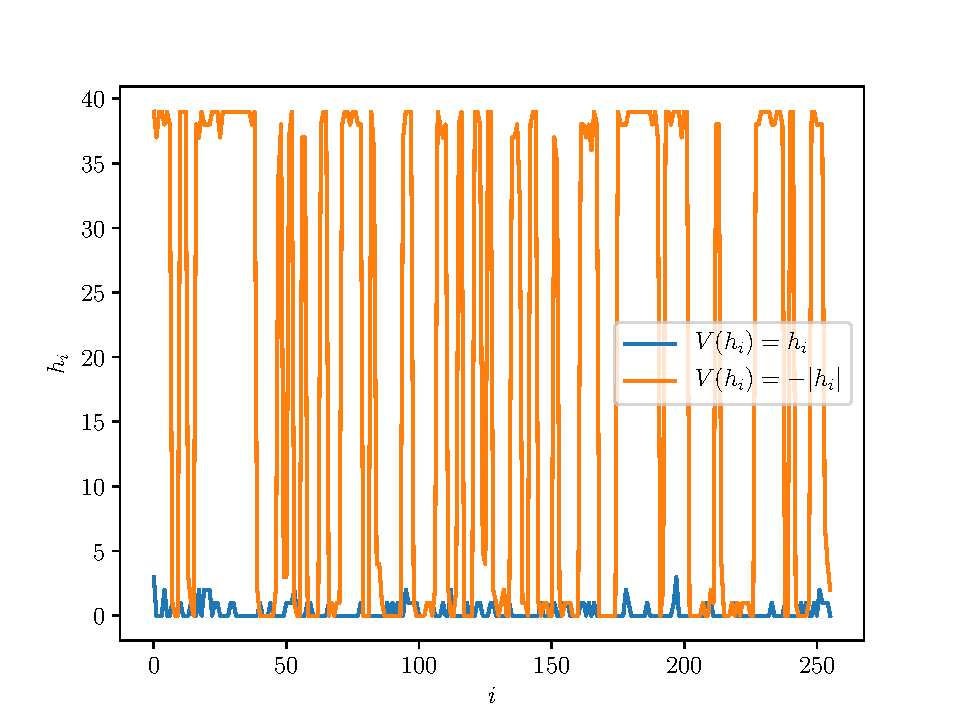
\includegraphics[width=\linewidth]{chap4/comp-potentiels-chimiques.pdf}
	\end{minipage}%Cyclin
	\begin{minipage}[t]{0.4\linewidth}
		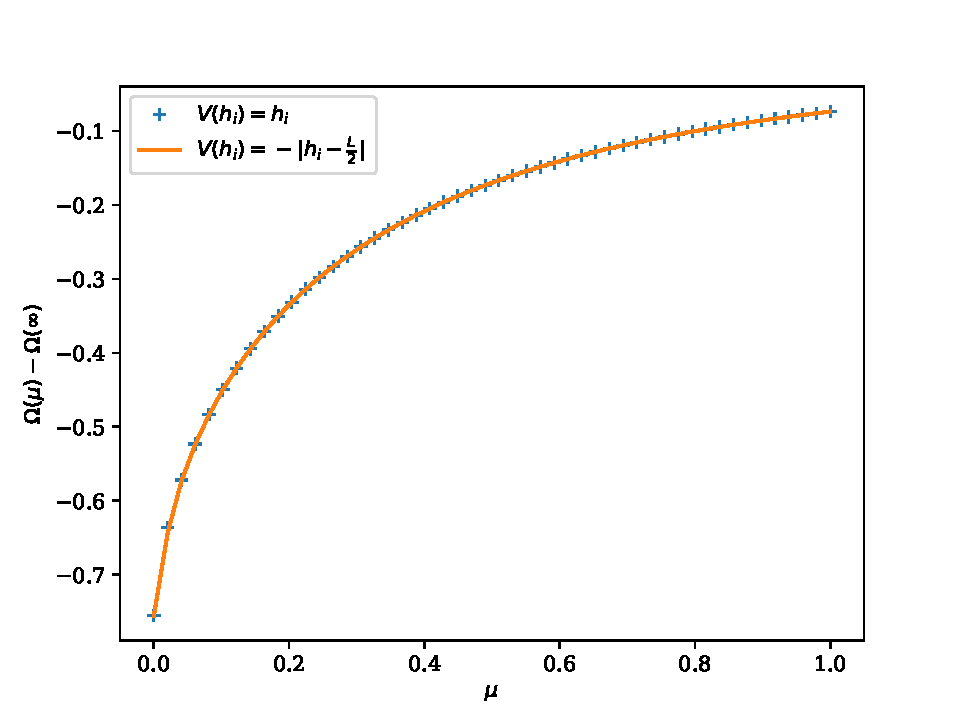
\includegraphics[width=\linewidth]{chap4/free-ene-potentiels.pdf}
	\end{minipage}
	\centering
	\begin{minipage}{0.4\linewidth}
    	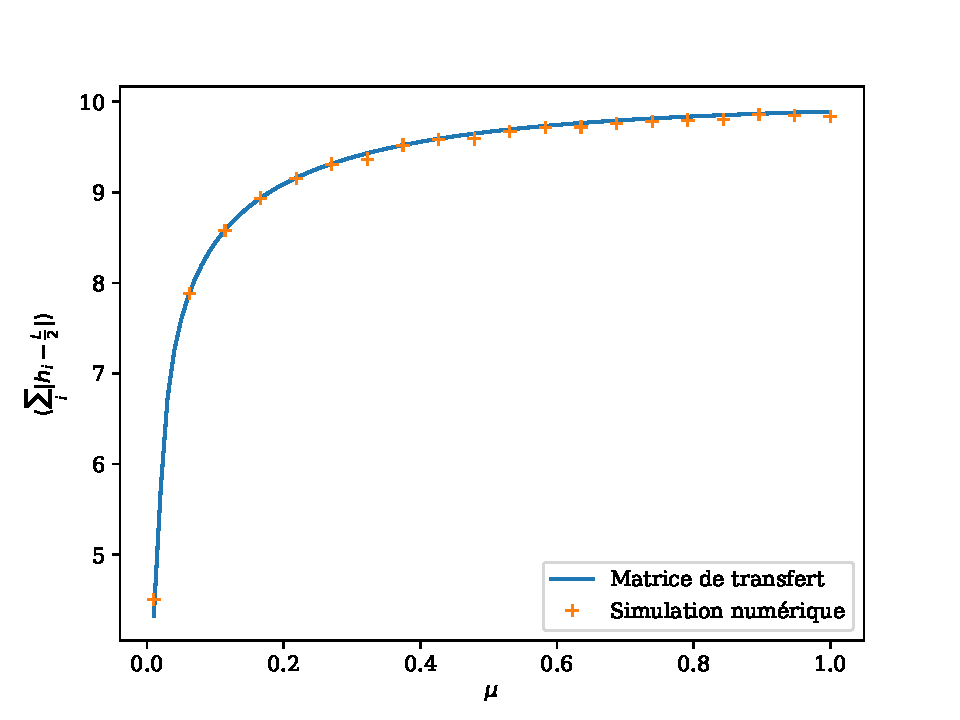
\includegraphics[width=\linewidth]{chap4/simu-tm-negstagged-l20.pdf}
	\end{minipage}
	\caption{Configuration possible du système à $\beta=1$ et $\mu$ élevé ($\mu=2$) pour les deux types de potentiel (gauche) ; énergie libre en fonction de $\mu$ à laquelle on a retiré l'énergie libre de la configuration limite pour les deux types de potentiel (droite) ; comparaison de l'observable $<\sum_i |h_i-\frac{L}{2}|>$ en fonction de $\mu$ entre la matrice de transfert et une simulation numérique avec $L=20$ pour $10^7$ étapes de Monte Carlo avec une dynamique de Glauber (bas). 
	{\color{red} pas clair, hyper vague. Insister sur la méthode numérique qui marche, proof of concept. Méthode, résultats originaux et proof of concept sont tout mélangés. Séparer}}
    \label{comp-potentiels-chimiques}
\end{figure}  

Dnas la limite $\mu \rightarrow \infty$, on a donc un système éparpillé à $h=0$ et $h=L$. On a la matrice de transfert
\begin{align}
T= e^{\beta \mu \frac{L}{2}}
  \begin{pmatrix}
    1 & e^{-\beta  J L} \\
    e^{-\beta  J L} & 1
  \end{pmatrix}
\end{align}
Les valeurs propres sont $\lambda_\pm = e^{ \beta \mu \frac{L}{2}}( 1 \pm e^{-\beta J L})$, ce qui nous donne dans la limite thermodynamique l'énergie libre 
\begin{align}
  \Omega(\mu \rightarrow \infty) = - \mu \frac{L}{2}
\end{align}
Il est donc aisé de calculer l'énergie libre pour un champ donné grâce à l'intégration
\begin{align}
        \Omega(\beta,L,\mu) = \Omega(\beta,L,\infty) + \int_{\mu}^\infty d\mu'  < \sum_i V(h_i) >_{\beta,L,\mu'} 
\end{align}
Cette méthode d'intégration est particulièrement adaptée aux modèles sur réseau où l'on connait la limite du système soumis à un potentiel extrême. Dans le cas du modèle SOS, on pourrait avoir envie de diagonaliser directement la matrice de transfert pour $\mu=0$, et ainsi obtenir
\begin{align}
        \Omega(\beta,L,\mu) =\Omega(\beta,L,0) + \int_{0}^\mu d\mu'  < \sum_i V(h_i) >_{\beta,L,\mu'} 
\end{align}
{\color{red} les longueurs de corrélation sont zéro, dans une limite est donnée uniquement par omega bulk+omefa surface.  fluctuations divergentes. Le système critique est $\mu \to 0$}
Pour petits champs, cette intégration est certes plus rapide, mais possède une limite divergente à $\mu=0$, qui correspond à une interface libre dont la magnétisation moyenne est une valeur sans intérêt, ce qui nous oblige à garder la limite $\mu \to \infty$.

 {\color{red} mettre en valeur figure 4.4, ÇA MARCHE avec le numérique, PLUS DE CONTEXTE !!}

{\color{red} Besoin MCIA pour faire Casimir Kawasaki, ajouter cisaillement }

%%%%%%%%%%%%%%%%%%%%%%%%%%%%%%%
    \section{Conclusion}
%%%%%%%%%%%%%%%%%%%%%%%%%%%%%%%	

Les systèmes statistiques dont la longueur de corrélation est similaire à la taille du système subissent des effets de taille finie qui affectent notablement ses propriétés. L'importance croissante des modes à faible longueur d'onde lorsque l'on réduit la taille du système, ainsi que les modifications des propriétés du mode de plus faible énergie, modifie l'énergie libre du système. Cette modification de l'énergie libre induit une force de Casimir intensive de la forme $f = -k_B T \frac{\partial \ln Z}{\partial L}$. Contrairement aux systèmes critiques, cette force a été très peu étudiée dans le modèle Solid-On-Solid, et n'exhibe aucune universalité simple. Le modèle Solid-On-Solid possède la particularité d'Être résolvable par la diagonalisation de la matrice de transfert. Cette méthode ne permet néanmoins que d'étudier l'effet Casimir que dans l'ensemble grand-canonique, puisqu'il n'est pas possible d'instaurer la contrainte $<h>=cte$ dans la matrice de transfert. 
Afin de pallier à ce probleme, une analyse Monte Carlo s'impose. La première méthode consiste à découplager progressivement une couche du système, afin que dans la limite où $L' \gg 1$, ce découplage s'apparente à la dérivée discrète de l'énergie libre. Néanmoins cette méthode a ses limites dans les modèles d'interface, puisqu'elle ne prend pas en compte l'absence d'énergie de bulk dans nos modèles. 
Une seconde méthode est d'intégrer par rapport au paramètre d'ordre $<h>$. Cependant, par définition de la dynamique de Kawasaki, cette méthode est vouée à l'échec. Nous avons développé un modèle possédant un hamiltonien produisant dans l'ensemble grand-canonique des résultats très similaires, que l'on a pu extrapoler pour l'ensemble canonique. 
{\color{red} Ajouter résultats avec cisaillement.}